\subsection{Command Pattern}

The Command pattern is described in \cite{GangOf4} as a behavioral pattern that 
encapsulates actions into objects. Each object is a representation of the 
operation. Thus, every command object is a self-contained implementation of the
action. In using this pattern, the system can provide an abstraction of the 
actions or commands. This pattern separates the knowledge of the implementation
of a command from the host program. In this way, the host only needs to execute
a generic command, with no regard to the implementation of the actual command. 
Any new command objects that are created in the future can be handled in the 
same way the other command objects are, eliminating the need to manipulate code
to handle the new commands.

The Command pattern involves a \texttt{Command} interface and \texttt{Command} 
objects, as shown in Figure~\ref{command}. Each of the \texttt{Command} objects
implements the \texttt{Command} interface, which contains a method called 
\texttt{execute()}. Every \texttt{Command} object must implement the 
\texttt{execute()} method. This method contains the actual implementation of the
command \cite{GangOf4}. 

\begin{figure}[htbp]
  \begin{center}
    \mbox{
      \subfigure[Command Pattern]{\scalebox{0.5}{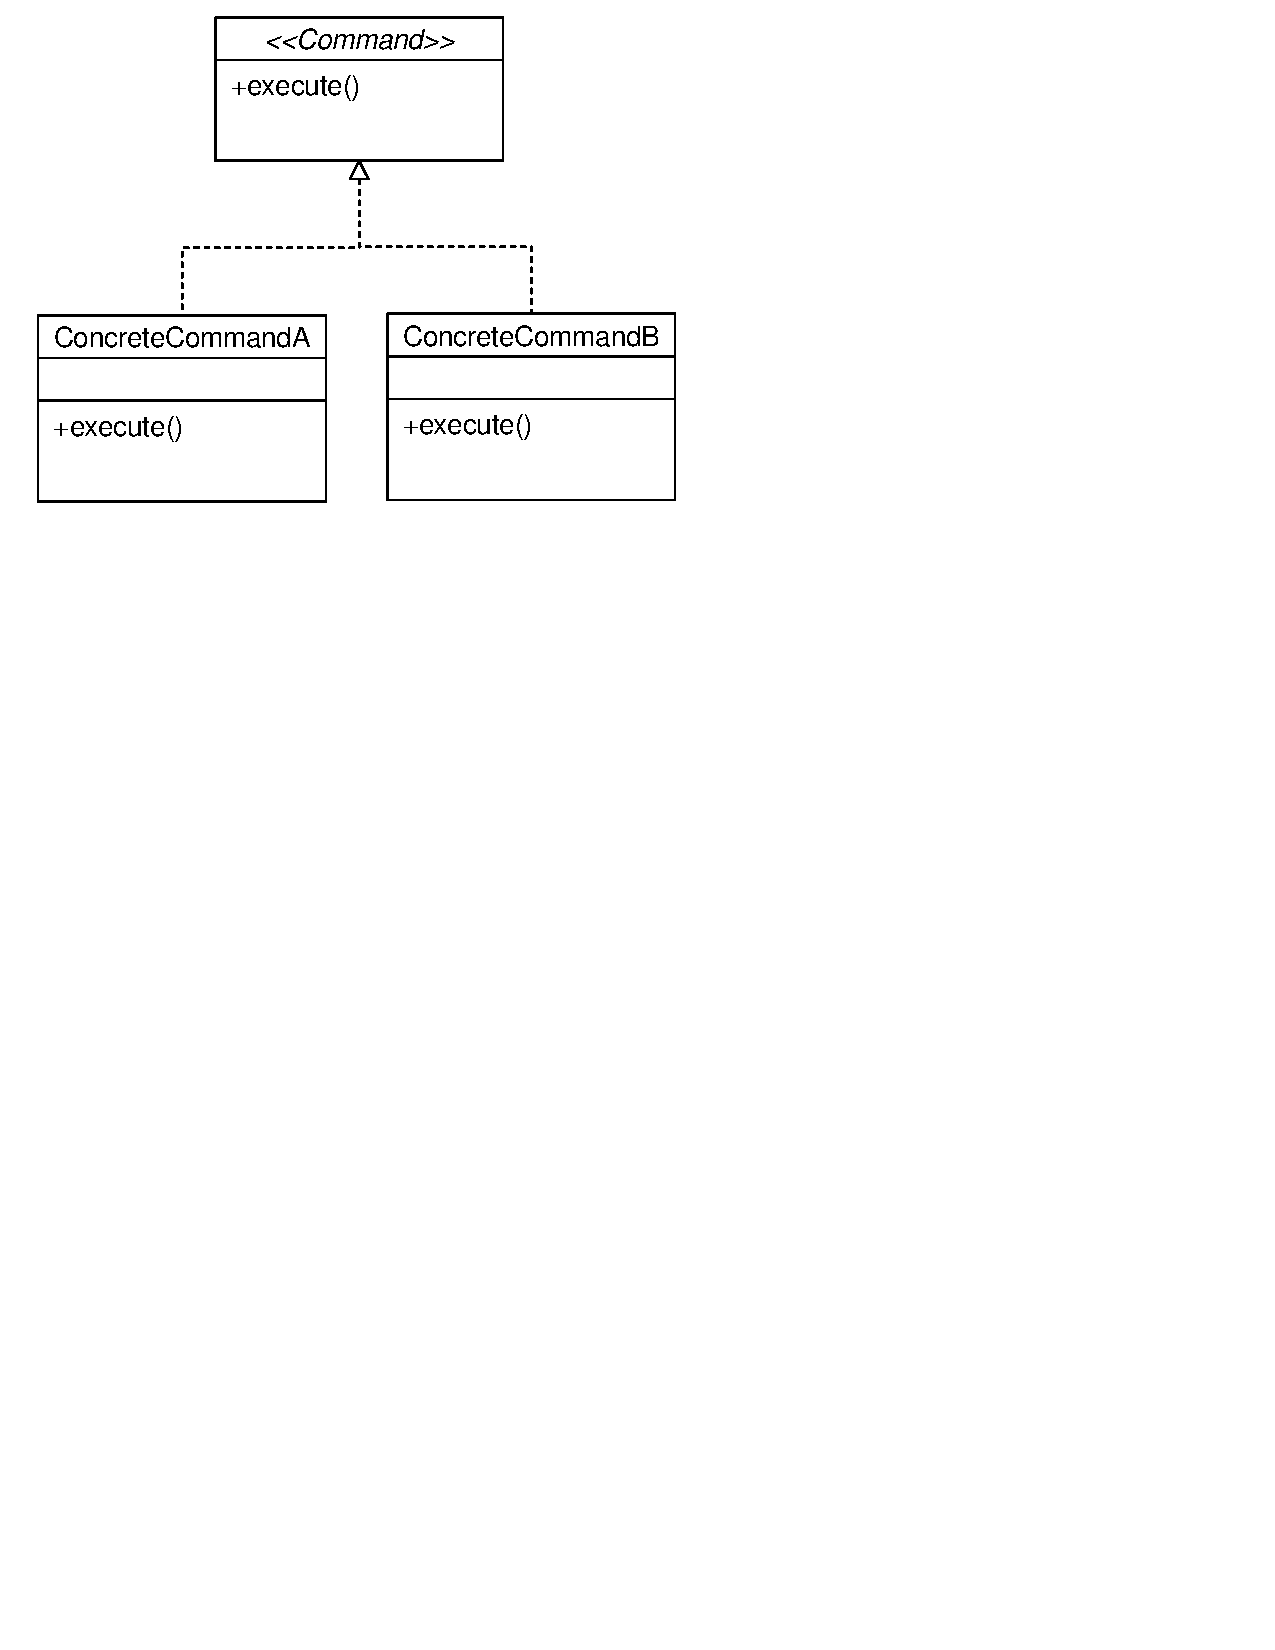
\includegraphics{./images/commandUML}}} \quad
      \subfigure[Coursebook's Use of Command Pattern]{\scalebox{0.5}{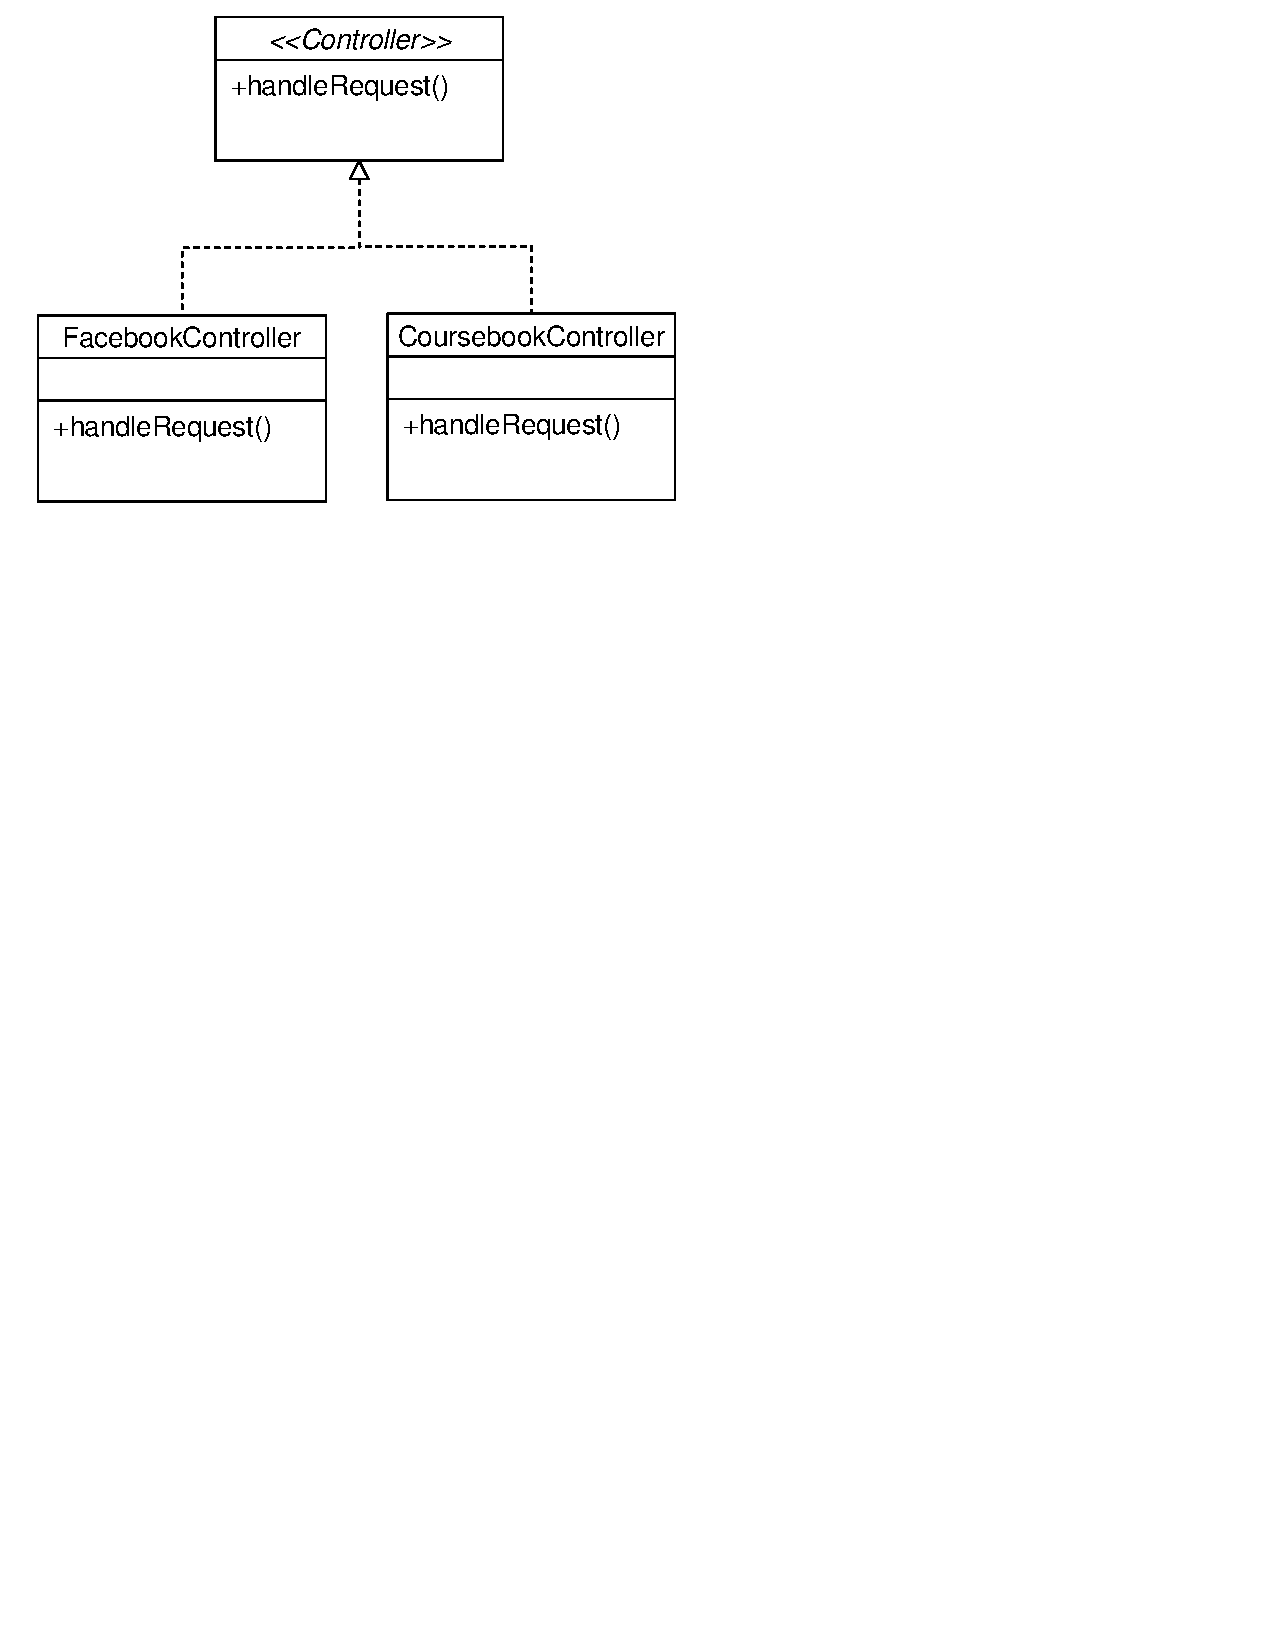
\includegraphics{./images/controllerUML}}}
    }
    \caption{The Command pattern}
    \label{fig:command}
  \end{center}
\end{figure}

Coursebook makes use of the  Command pattern in its controllers (see
Figure \ref{controllerUML}). There are two types of requests that Coursebook
handles: Facebook requests and Coursebook requests. Facebook requests are from
clients that log into Facebook and request classes based upon their Facebook 
interests. Coursebook requests are from clients that manually enter their 
interests to request relevant classes. Using the Command pattern to encapsulate
these two types of requests eliminates the need for the Coursebook system to 
differentiate how to handle these two types of requests. Coursebook defines a
\texttt{Controller} interface, which represents the \texttt{Command} interface 
in the Command pattern. This interface defines a method
\texttt{handleRequest()}. Two classes, \texttt{FacebookController} and
\texttt{CoursebookController}, implement the \texttt{Controller} interface and
implement the \texttt{handleRequest()} method. Each of the concrete controllers
define the implementation for that type of request. When Coursebook handles a
request, it simply calls the \texttt{handleRequest()} method, oblivious to the 
two different types of commands that can be invoked from that method. This 
implementation abstracts the implementation details of the two controllers and
allows for the addition of request handlers with minimal code refactoring.
